\documentclass[11pt,a4paper]{article}

% Packages
\usepackage{fontspec}
\setmainfont{Hiragino Mincho ProN}
\setsansfont{Hiragino Kaku Gothic ProN}
\setmonofont{Menlo}
\usepackage{iftex}
\ifXeTeX
  \XeTeXlinebreaklocale "ja"
  \XeTeXlinebreakskip=0pt plus 1pt minus 0.1pt
\fi
\usepackage{amsmath,amssymb,amsthm}
\usepackage{graphicx}
\usepackage{hyperref}
\usepackage{booktabs}
\usepackage{xcolor}
\usepackage[margin=2.5cm]{geometry}
\usepackage[numbers]{natbib}
\usepackage[protrusion=true,expansion=false]{microtype}

% Theorem environments
\newtheorem{theorem}{定理}[section]
\newtheorem{lemma}[theorem]{補題}
\newtheorem{proposition}[theorem]{命題}
\newtheorem{definition}[theorem]{定義}

% Shortcuts
\newcommand{\mc}{\mu_c}
\newcommand{\Neff}{N_{\text{eff}}}
\newcommand{\Ssolve}{S_{\text{solve}}}
\newcommand{\Pfound}{P(\text{found})}
\newcommand{\PSAT}{P(\text{SAT})}
\newcommand{\PfSAT}{P(\text{found}\mid\text{SAT})}

% Title
\title{構造パラメータ$\delta$による計算コストの予測：\\ランダム3-SATにおける存在と発見の分離}
\author{Akihito Sunagawa\thanks{akihito.sunagawa@gmail.com}}
\date{2026年3月}

\begin{document}

\maketitle

\begin{abstract}
解が\emph{存在する}かどうかと、アルゴリズムがそれを\emph{発見できる}かどうかは、異なるメカニズムに支配される別個の問題である。
ランダム3-SATにおいて、第一モーメント法は
$\PSAT \approx \Neff \cdot e^{-\delta}$
を与える。ここで$\delta = \alpha n |\!\ln(7/8)|$は節密度の再パラメータ化（第一モーメント法における指数）である。これは存在を特徴づけるが、発見については何も語らない。

本稿では計算予算$\mu$（ソルバー操作数）を導入し、条件付き成功確率$\PfSAT$が$\mu / \mc(\delta)$の関数として乗法的に分解可能かを問う。

$n = 100$--$300$変数、$\alpha = 3.0$--$4.0$のインスタンスに対する3つのソルバーファミリー（CDCL、WalkSAT、ランダム探索）の実験から、3つの知見が得られた。
(1)~中央値ランタイムは$\mc \propto e^{c\delta}$でスケールし、\emph{感応度指数}$c$はソルバー依存である：
$\alpha \geq 3.5$のフロアフリー領域で
CDCLでは$c \approx 0.24$、
WalkSATでは$c \approx 0.21$、
ランダム探索では$c = 1.0$（厳密）
（ソルバーのスタートアップオーバーヘッドが支配的な$\alpha = 3.0$を含めたフィットではそれぞれ$c = 0.25$および$0.18$；第\ref{sec:mu_c}節参照）。
(2)~比$\mu/\mc$は有効な正規化変数である：
両ソルバーとも$\mu/\mc = 1$付近で単調な遷移を示し、$x_0 \approx 0$であるが、遷移の形状は14--15\%異なる（シグモイドおよびワイブルフィットの両方でモデル非依存）。
(3)~$c_{\text{CDCL}} > c_{\text{WalkSAT}}$の順序は問題サイズ（$n = 100$--$300$）にわたってロバストであるが、共通の節密度範囲（$\alpha = 3.5$--$4.0$）で測定すると両推定値とも中程度の$n$依存性を示す（CDCLで${\sim}18\%$、WalkSATで${\sim}7\%$の範囲）。
$n \leq 200$で訓練し$n = 300$を予測するクロス$n$予測テストは、$\mc$が3桁にわたる範囲で2倍精度（対数空間でRMSE $= 0.73$）を達成する（付録\ref{app:prediction}）。

パラメータ$\delta$は存在（$c=1$、数学的恒等式）と発見（$c < 1$、アルゴリズム依存）の両方を支配するが、感応度は質的に異なる。
注目すべきことに、$c$は$\delta$への感応度を測るものであり、効率を測るものではない：WalkSATは最も小さい$c$をもつが最も大きい絶対コストをもつ。これは低い感応度が構造の活用ではなく構造の無視から生じうることを意味する。

\medskip
\noindent\textbf{キーワード：} ランダム3-SAT、計算予算、存在--発見分離、第一モーメント法、ソルバー比較、感応度指数
\end{abstract}

%=============================================
\section{序論}
\label{sec:intro}

ランダム$k$-SATの充足可能性閾値は、組合せ論および統計物理学において最もよく研究された現象の一つである\cite{MPZ2009}。
キャビティ法とその厳密な対応物は、解が存在しなくなる臨界節密度$\alpha_c$を精度を高めながら決定してきた\cite{Achlioptas2008,Ding2015}。
これらの結果は\emph{存在}の問題に答える：与えられた節対変数比$\alpha$に対し、充足割り当ては高い確率で存在するか？

相補的な問題はあまり形式的な注目を受けていない：解が\emph{存在する}として、それを\emph{発見する}にはどれだけの計算が必要か？
最悪ケース計算量理論は上界を提供し（例えば$k$-SATに対するSch\"oningの$(2(1-1/k))^n$\cite{Schoening1999}）、経験的研究はランタイム分布（RTD）の裾の重さを記録している\cite{Gomes2000,Coarfa2003,Hoos1999,Frost1997}。
Cocco and Monasson\cite{CoccoMonasson2001}はDPLLの計算コストを節密度の関数として解析的に導出し、典型的な計算量が$\alpha$依存のレートで指数的に増大することを示した。
RTDは与えられた時間予算内で解を見つける確率を特徴づけ、アルゴリズム選択やリスタート方策設計に使われてきた\cite{Hoos1999}。
しかし、RTDを第一モーメント法の構造パラメータ$\delta$に接続し、$\delta$を用いて中央値ランタイムが節密度にわたってどうスケールするかを予測する枠組みは存在しない。

この空隙を、恒等式としては自明だが定量的プログラムとしては非自明な分解を通じて定式化する：
\begin{equation}
\label{eq:decomposition}
\Pfound = \underbrace{\PSAT}_{\text{存在}} \;\times\;
          \underbrace{\PfSAT}_{\text{発見}}.
\end{equation}
左の因子は第一モーメント法によりよく特徴づけられている。
右の因子---\emph{発見確率}---が我々の測定対象である。

我々の中心的知見は、同一の構造パラメータ$\delta$（節密度$\alpha$の再パラメータ化であり、第一モーメント法における指数に等しい）が両因子を支配するが、その強さが異なるということである：
\begin{itemize}
\item \textbf{存在：} $\PSAT \approx \Neff \cdot e^{-\delta}$、$c = 1$（数学的恒等式）。
\item \textbf{発見：} 計算コストの中央値は$\mc \propto e^{c\delta}$でスケールし、$c < 1$であり、$c$はソルバーファミリーに依存する。
\end{itemize}
感応度指数$c$は、ソルバーのコストが構造的複雑度$\delta$の増加にどれだけ強く応答するかを測る。
これは効率の尺度では\emph{ない}：
CDCL（$c \approx 0.24$）はWalkSAT（$c \approx 0.21$）より$\delta$に対する感応度が高いが、絶対コストでは10--50倍高速である。
洗練度は感応度を増加させるのであり、減少させるのではない。


%=============================================
\section{枠組み}
\label{sec:framework}

\subsection{存在：第一モーメントベースライン}

$n$個の変数と$m = \alpha n$個の節をもつランダム3-SATインスタンスを考える。各節は一様ランダムに選ばれた3つのリテラルの選言である。
一様ランダム割り当てが単一の節を充足する確率は$k=3$に対して$1 - 2^{-k} = 7/8$である。
充足割り当ての期待数は
\begin{equation}
\label{eq:first-moment}
\mathbb{E}[\#\text{SAT}] = 2^n \cdot (7/8)^m
  = \exp\!\bigl(n\ln 2 - \delta\bigr),
\end{equation}
ここで
\begin{equation}
\label{eq:delta}
\delta \;\equiv\; \alpha\, n\, |\!\ln(7/8)|
  \;=\; m \cdot |\!\ln(7/8)|
\end{equation}
は節数$m$（あるいは与えられた$n$における節密度$\alpha$）の再パラメータ化であり、$|\!\ln(7/8)| \approx 0.134$ナット/節である。
これはアニール化（レプリカ対称）近似である；アニール化閾値$\alpha_c^{(1)} \approx 5.19$と真の閾値$\alpha_c \approx 4.27$\cite{MPZ2009}の間の20\%の差は、よく理解されているがここでの目的には無関係なレプリカ対称性の破れの補正を反映している。

式\eqref{eq:first-moment}はアニール化枠組みの中での数学的恒等式である。
パラメータ$\delta$は\emph{新しい}量ではない：単に$m \cdot |\!\ln(7/8)|$であり、インスタンスの仕様から計算可能で、第一モーメント法における指数と同一である\cite{MPZ2009}。
新しいのは、$\delta$が\emph{計算コスト}をもソルバー依存の比例定数で支配するという経験的観察である（第\ref{sec:mu_c}節）。

\subsection{発見：計算予算の導入}

$\mu$をソルバーが利用可能な計算予算（ソルバー固有の単位で測定：CDCLではコンフリクト数、WalkSATではフリップ数、ランダム探索ではトライアル数）とする。
\textbf{発見確率}を
\begin{equation}
\label{eq:ssolve}
\Ssolve(\delta, \mu) \;\equiv\; \PfSAT
\end{equation}
と定義する。これは、インスタンスが充足可能であることを条件として、ソルバーが予算$\mu$以内に充足割り当てを見つける確率である。
これは充足可能インスタンスに限定したランタイム分布（RTD）\cite{Hoos1999,Frost1997}の累積分布関数である。

我々の仮説は、$\Ssolve$が中央値ランタイム$\mc(\delta)$を通じて\textbf{乗法的分離}を許容するというものである：
\begin{equation}
\label{eq:separation}
\Ssolve(\delta, \mu) = f\!\left(\frac{\mu}{\mc(\delta)}\right),
\end{equation}
ここで$f$は単調増加関数（CDFに類似した遷移）であり、中央値ランタイムは指数的にスケールする：
\begin{equation}
\label{eq:mu_c}
\mc(\delta) = A \cdot e^{c\,\delta}.
\end{equation}
ここで$c$は\textbf{感応度指数}---$\delta$の1単位あたりの計算コストの増加率---であり、$A$は単位依存の切片（ソルバー実装の絶対速度を吸収する）である。

\paragraph{なぜ指数形式か？}
式\eqref{eq:mu_c}の指数形式は恣意的なモデリング選択ではない。
制約がコストに独立に寄与するならば---すなわち$\mc(\delta_1 + \delta_2) = \mc(\delta_1) \cdot [\mc(\delta_2)/A]$---コーシーの関数方程式$g(\delta_1 + \delta_2) = g(\delta_1) \cdot g(\delta_2)$（$g = \mc/A$、$g(0) = 1$、$g$は連続かつ単調増加）の一意解は$g(\delta) = e^{c\delta}$（$c > 0$）である\cite{Aczel1966}。
換言すれば、式\eqref{eq:mu_c}は制約の独立な蓄積と両立する\emph{唯一の}連続的スケーリング則である。
パラメータ$c$はこの一意解のスケール定数であり、構造的複雑度に対するソルバーの固有感応度を測る。
（この特徴づけ定理のLean 4による形式検証は補足リポジトリで利用可能である。）

\paragraph{感応度指数の適用範囲}
本稿を通じて、$c$は\emph{固定された}問題サイズ$n$において節密度$\alpha$を変化させることで測定される。
すなわち、$\delta$は$\alpha$と$n$を混合する普遍座標としてではなく、（与えられた$n$における）$\alpha$の再パラメータ化として機能する。
$n$に関するランタイムのスケーリング（$\alpha$固定）は$\alpha$に関するスケーリング（$n$固定）と質的に異なりうるため、この区別は重要である。
特に、確率的局所探索ソルバーは相転移において$n$に対して多項式的にスケールすることが知られており\cite{MuHoos2015}、これは$\delta = \alpha n|\!\ln(7/8)|$を両軸にわたる単一の指数的予測子として扱うことと両立しない。
第\ref{sec:asymmetry}節でこの非対称性を詳細に議論する。

重要なことに、$c$は$\mu$の再スケーリングに対して不変である：$\mu \to k\mu$ならば$A \to kA$であるが、$\ln \mc$ vs.\ $\delta$の傾き$c$は不変である。
これにより$c$は\emph{実装}の性質ではなく\emph{アルゴリズム}の性質となる。

\paragraph{3つの検証可能な仮説}
\begin{description}
\item[H1（完全分離）：] $\mc$は$\alpha$（したがって$\delta$）に依存しない。異なる$\alpha$値が同一のランタイム分布をもたらすことになる。
\item[H2（$\mc$結合分離）：] $\mc$は式\eqref{eq:mu_c}を通じて$\delta$に依存し、$\mu/\mc$が異なる$\alpha$値からの生存曲線を単一の関数$f$に折りたたむ。
\item[H3（非分離）：] $\mu$のいかなる再スケーリングも異なる$\alpha$値からの曲線を折りたたむことができない。
\end{description}

\paragraph{$c = 1$ベースライン}
ランダム探索（割り当てを一様ランダムにサンプリングし全節を検査、これを繰り返す）の場合、解を見つけるまでの期待トライアル数は$2^n / \#\text{SAT} = e^{\delta} / \Neff$に等しい。
したがって$\mc^{\text{random}} \propto e^{\delta}$であり、$c = 1$が厳密に成り立つ。
これは近似ではなく、第一モーメント恒等式\eqref{eq:first-moment}の帰結である。
$c < 1$をもつ任意のソルバーは、正確な意味で、構造のないベースラインよりも構造的複雑度の1単位あたりのコスト増加が少ない。


%=============================================
\section{実験設定}
\label{sec:experiments}

\subsection{インスタンス生成}

$n \in \{100, 200, 300\}$変数、節密度$\alpha \in \{3.0,\; 3.5,\; 3.86,\; 4.0\}$のランダム3-SATインスタンスを生成する。
$\alpha > 4.2$は除外する：充足可能インスタンスの割合が充足可能性閾値$\alpha_c \approx 4.27$付近で急激に低下し、\emph{生存者バイアス}---高い$\alpha$で充足可能と判明したインスタンスは典型的な充足可能インスタンスより系統的に容易である---を導入するためである。
各$(n, \alpha)$ペアに対して100--200インスタンスを生成し、充足可能と確認されたもの（無制限CDCLランによる）のみを保持する。

\subsection{ソルバー}

3つのソルバーファミリーがアルゴリズムの洗練度の範囲をカバーする：

\begin{description}
\item[CDCL（PySAT経由MiniSat）：]
  リスタート付きコンフリクト駆動節学習\cite{MarquesSilva1999}。
  予算単位：\emph{コンフリクト}（含意グラフにおける状態遷移）。
  予算範囲：$10^2$--$10^5$。

\item[WalkSAT（純粋Python、リスタート付き）：]
  ノイズパラメータ0.5および定期的リスタート付き確率的局所探索\cite{SKC1994}。
  予算単位：\emph{フリップ}（単一変数の再割り当て）。
  予算範囲：$10^3$--$10^6$。

\item[ランダム探索：]
  一様ランダム割り当て、全節を検査、繰り返し。
  予算単位：\emph{トライアル}。
  $c = 1$の理論的ベースラインとして機能する。
\end{description}

\subsection{測定プロトコル}

各インスタンスに対してまず無制限ソルブを実行し真のランタイムを取得する（$\mc$を各$\alpha$におけるインスタンス間の中央値として定義）。
次に対数等間隔の予算値において$\Ssolve$を測定し、各予算内に解かれたSATインスタンスの割合を記録する。

条件付き分析$\PfSAT$（$\Pfound$ではなく）が不可欠である：$\alpha = 4.0$では約8\%のインスタンスが充足不可能であり、それらを含めると存在閾値と発見遷移が混同される。


%=============================================
\section{結果}
\label{sec:results}

\subsection{$\mc \propto e^{c\delta}$：感応度指数}
\label{sec:mu_c}

図\ref{fig:mu_c}に3つのソルバーファミリーについて$\ln \mc$対$\delta$を示す。
4つの$\alpha$値に対する線形回帰は以下を与える：

\begin{figure}[ht]
\centering
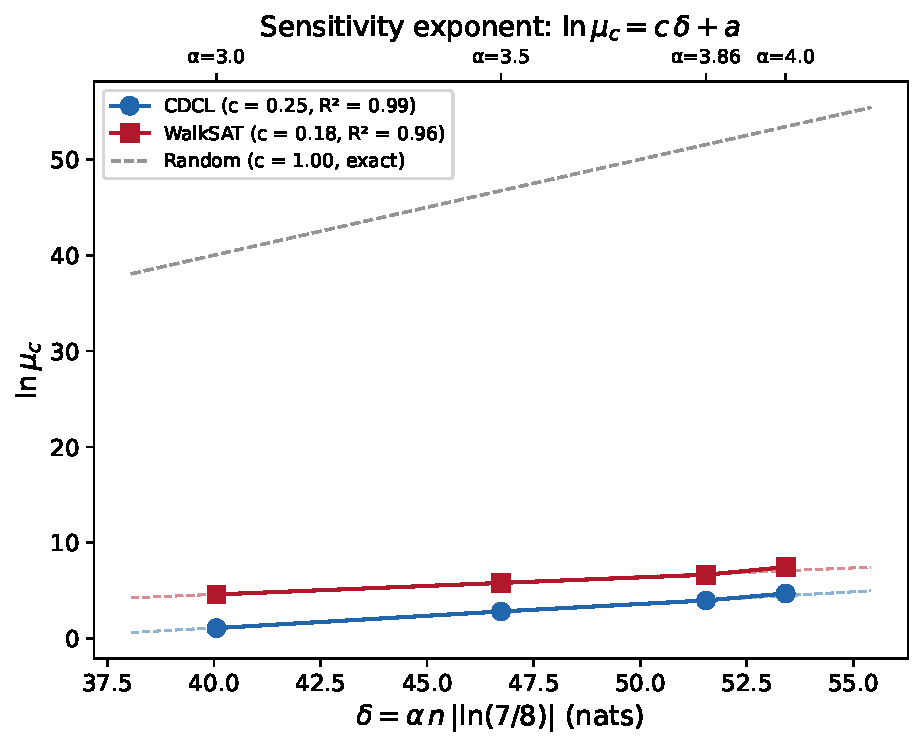
\includegraphics[width=0.85\textwidth]{fig1_sensitivity_exponent.pdf}
\caption{3つのソルバーファミリーに対する$\ln \mc$対$\delta = \alpha n |\!\ln(7/8)|$（$n = 100$、$\alpha = 3.0$--$4.0$）。
破線：線形フィット$\ln \mc = c\delta + a$。
フィットはソルバーのスタートアップオーバーヘッドがフロア効果を生む$\alpha = 3.0$を含む（第\ref{sec:discussion}節）；$\alpha \geq 3.5$に限定すると$c \approx 0.24$（CDCL）および$c \approx 0.21$（WalkSAT）となる。}
\label{fig:mu_c}
\end{figure}

\begin{table}[h]
\centering
\begin{tabular}{lcccc}
\toprule
ソルバー & $c$ & 95\% CI & $R^2$ & 備考 \\
\midrule
CDCL（コンフリクト）   & 0.25  & $[0.24,\; 0.29]$ & 0.99  & \\
WalkSAT（フリップ）    & 0.18  & $[0.17,\; 0.22]$ & 0.96  & \\
ランダム（トライアル）    & 1.0   &  ---              &  ---  & 厳密（式\ref{eq:first-moment}） \\
\bottomrule
\end{tabular}
\caption{$\ln \mc = c\delta + a$からの感応度指数$c$（$n = 100$、$\alpha = 3.0$--$4.0$）。
95\% CIはブートストラップパーセンタイル区間（200インスタンス$\times$ 10\,000リサンプル）。
CIは重複せず、$c_{\text{CDCL}} > c_{\text{WalkSAT}}$の順序が統計的に有意であることを確認する。
注：これらの推定値はフロア効果が$c$にバイアスを与える$\alpha = 3.0$を含む（第\ref{sec:discussion}節）；$\alpha \geq 3.5$に限定すると$c \approx 0.24$（CDCL）および$c \approx 0.21$（WalkSAT）となる。}
\label{tab:c_values}
\end{table}

傾き$c$は単位の再スケーリングに対して不変であり（$\mu \to k\mu$は切片$a$をシフトするが傾きは変えない）、CDCLとWalkSATの差はコンフリクトとフリップを比較するアーティファクトではない。

\paragraph{$c$の$n$依存性}
$\alpha$回帰を$n = 100$、$200$、$300$で繰り返すと（付録\ref{app:n_scaling}）、推定される$c$は節密度範囲に依存することが明らかになる。
$\alpha = 3.0$ではCDCLの中央値コンフリクト数はすべての$n$で3--8であり---指数的スケーリングではなくソルバーのスタートアップオーバーヘッドに支配されている。
この\emph{フロア効果}は線形フィットにバイアスを与える：$\alpha = 3.0$を含めると$c \approx 0.19$であるのに対し、$\alpha \geq 3.5$に限定すると$c \approx 0.24$となる（付録\ref{app:alpha_density}の8点精密フィットからの$c = 0.24$も参照）。

共通の節密度範囲（$\alpha = 3.5$--$4.0$、局所傾き）で測定すると、両ソルバーとも中程度の$n$依存性を示す：
CDCLは$n = 100, 200, 300$で$c = 0.26, 0.22, 0.24$、WalkSATは$c = 0.21, 0.21, 0.20$（範囲はそれぞれ18\%および7\%）。
$c_{\text{CDCL}} > c_{\text{WalkSAT}}$の順序はテストしたすべての$n$で成り立ち、$n \geq 200$ではブートストラップ95\% CIが重複しない（$P > 0.99$）；$n = 100$では2点フロアフリー傾きのCIが広く、差は有意でない（$P = 0.76$）。
差（0.02--0.05）は全範囲推定値が示唆するよりも小さい。
WalkSATの$n$依存性はさらに、線形$\delta$モデルが切片だけでは吸収できない多項式$n$スケーリングを反映している（第\ref{sec:asymmetry}節および付録\ref{app:n_scaling}参照）。

\paragraph{解釈}
$c_{\text{WalkSAT}} < c_{\text{CDCL}} < c_{\text{Random}}$の順序は一見驚くべきものである：最も効率的なソルバー（CDCL）がWalkSATよりも$\delta$に対して\emph{より高い}感応度をもつ。
これは$c < 1$の質的に異なる2つのメカニズムを反映している：
\begin{itemize}
\item CDCL（$c \approx 0.24$）：節学習が制約構造を能動的に活用し、効率\emph{と}その構造への感応度の両方を高める。
\item WalkSAT（$c \approx 0.21$）：局所探索は大域的な制約構造をほとんど無視するため、$\delta$への応答性が低い---しかし絶対コストも高い（$\mc$はCDCLの10--50倍）。
\end{itemize}
したがって$c$と絶対効率（$1/A$）は独立な2つの軸である：$c$はコストが$\delta$とともに\emph{どれだけ}増加するかを測り、$A$は$\delta = 0$でのベースラインコストを測る。


\subsection{正規化変数としての$\mu/\mc$}
\label{sec:normalization}

図\ref{fig:transition}にCDCLおよびWalkSATについて4つの$\alpha$値にわたる$\ln(\mu/\mc)$の関数としての$\Ssolve$を示す。

\begin{figure}[ht]
\centering
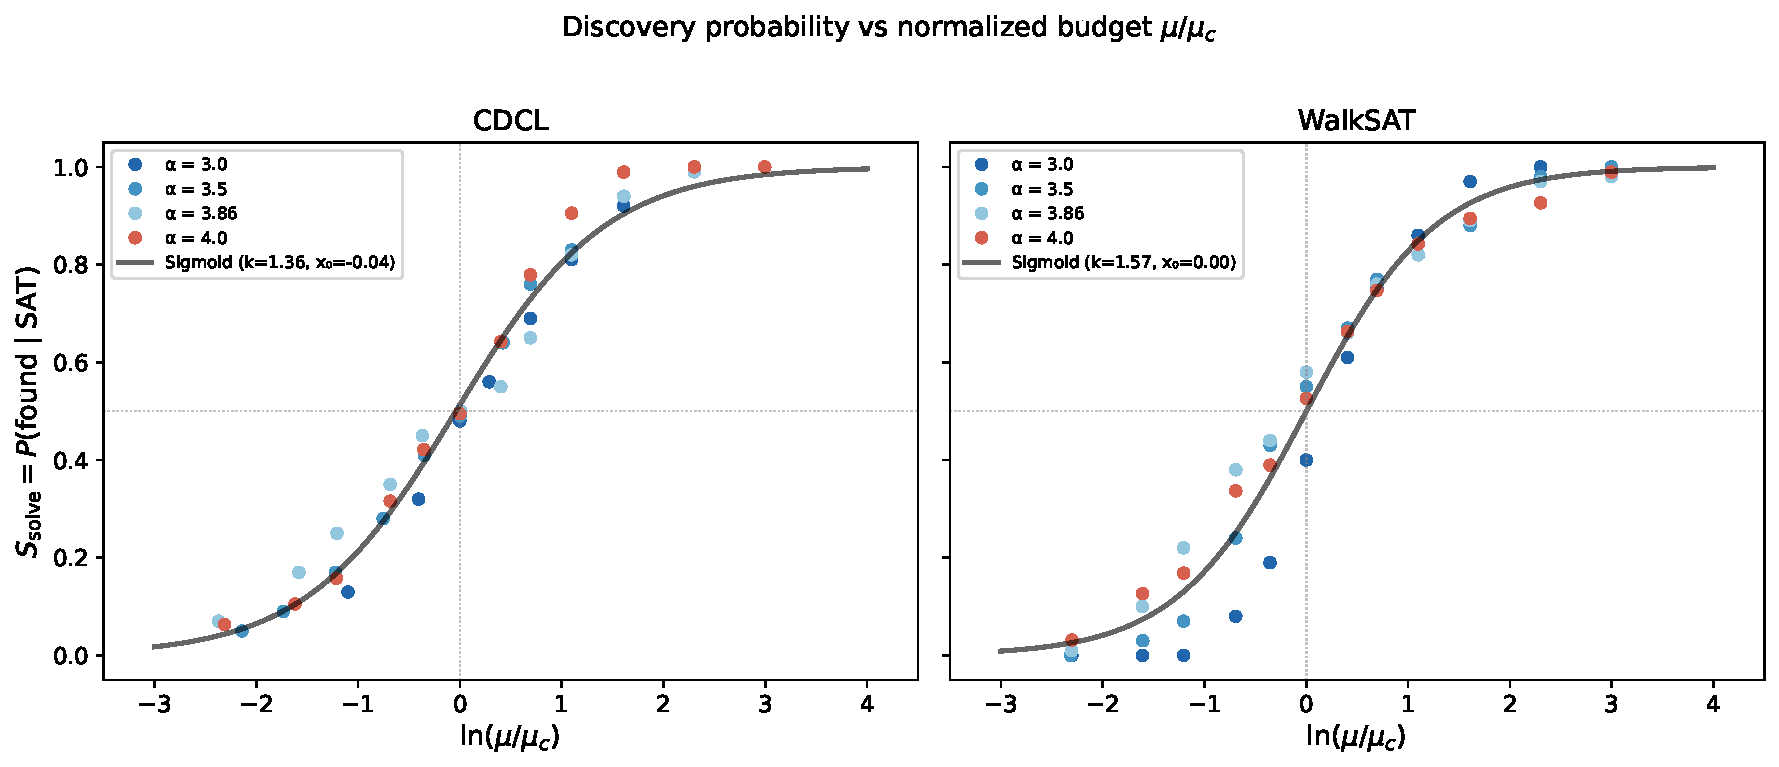
\includegraphics[width=\textwidth]{fig2_transition_curves.pdf}
\caption{CDCLl（左）およびWalkSAT（右）の発見確率$\Ssolve$対$\ln(\mu/\mc)$、4つの$\alpha$値（$n = 100$）。
実線：シグモイドフィット。
両ソルバーとも$\mu/\mc = 1$（$x_0 \approx 0$）付近で遷移し、$\mc$が自然な予算スケールであることを検証する。
急峻度$k$は14\%異なる（CDCL: 1.36、WalkSAT: 1.57）。}
\label{fig:transition}
\end{figure}

ロジスティック（シグモイド）モデル$\Ssolve = [1 + \exp(-k(\ln(\mu/\mc) - x_0))]^{-1}$のフィットは以下を与える：

\begin{table}[h]
\centering
\begin{tabular}{lcccc}
\toprule
フィット & $k$ & $x_0$ & $R^2$ & $n_{\text{pts}}$ \\
\midrule
CDCLのみ     & 1.36 & $-0.04$ & 0.985 & 45 \\
WalkSATのみ  & 1.57 & $ 0.00$ & 0.972 & 48 \\
結合      & 1.46 & $-0.01$ & 0.976 & 93 \\
\bottomrule
\end{tabular}
\caption{遷移曲線のシグモイドフィットパラメータ。
両ソルバーとも$x_0 \approx 0$であり、$\mc$（中央値ランタイム）が50\%遷移点を自然に示すことを確認する。
急峻度$k$は14\%異なる。}
\label{tab:sigmoid}
\end{table}

2つの重要な観察：
\begin{enumerate}
\item 両ソルバーとも$x_0 \approx 0$であり、50\%成功確率が$\mu = \mc$付近で生じることを意味する。
  これにより中央値ランタイムが計算予算の自然なスケールとして検証される。
\item 急峻度パラメータ$k$は14\%異なる（CDCL: 1.36、WalkSAT: 1.57）。
  普遍的なスケーリング関数を\emph{主張しない}；代わりに、$\mu/\mc$がソルバー固有の特徴を保持する遷移形状をもつ有効な正規化変数であることを報告する。
\end{enumerate}

$\mu/\mc = 1.0$において、CDCLは4つすべての$\alpha$値で$\Ssolve = 0.48$--$0.50$を達成し（ほぼ完全な折りたたみ）、WalkSATは$\Ssolve = 0.40$--$0.58$を示す（より散らばりが大きい）。
これはコンフリクトがフリップよりも$\mu$のより自然な単位であることを示唆する。

\paragraph{モデル非依存性}
14\%の形状差がシグモイド関数形式のアーティファクトでないことを検証するため、ワイブルCDF $\Ssolve = 1 - \exp(-(\mu/\mc)^\beta)$もフィットした。
ワイブル形状パラメータはソルバー間で同等の15\%の差を示す（付録\ref{app:model}の表\ref{tab:weibull}）。
AIC比較により、最良フィットモデル自体がソルバー依存であることが明らかになった：CDCLではワイブル（$\beta = 0.93$）、WalkSATではシグモイド。
したがって形状差はランタイム分布の真の性質であり、フィッティングのアーティファクトではない。


\subsection{ランタイムの異質性}
\label{sec:heterogeneity}

ワイブル形状パラメータ$\beta$はランタイム分布の構造に対する洞察を提供する：

\begin{table}[h]
\centering
\begin{tabular}{lccc}
\toprule
ソルバー & $c$ & ワイブル$\beta$ & $\Delta\beta$（vs ランダム） \\
\midrule
ランダム   & 1.00 & $0.87 \pm 0.05$ & ベースライン \\
CDCL     & 0.25 & 0.93 & $+0.06$ \\
WalkSAT  & 0.18 & 1.10 & $+0.23$ \\
\bottomrule
\end{tabular}
\caption{ソルバー別のワイブル形状パラメータ。
ランダム探索の$\beta < 1$はインスタンス間の異質性を反映する（指数分布の混合の既知の性質）。
$\Delta\beta$は各ソルバーがインスタンスの難易度をどの程度均質化するかを測る。}
\label{tab:beta}
\end{table}

ランダム探索ベースラインの$\beta = 0.87 < 1$は異常ではない：インスタンス間で成功確率が異なる指数分布の混合の期待されるシグネチャである（混合のハザード率減少性）。
このベースラインに対する各ソルバーの$\Delta\beta$は、アルゴリズムがインスタンスの難易度をどの程度\emph{均質化する}かを測る。

$c$と$\beta$は単調な関係にないことに注意する（$c$：ランダム $>$ CDCL $>$ WalkSAT；$\beta$：WalkSAT $>$ CDCL $>$ ランダム）：これらはソルバーと構造の相互作用の異なる側面を測定している。
感応度$c$はコストが$\delta$とともにどう\emph{スケールする}かを捉え、$\Delta\beta$はソルバーが難易度の異なるインスタンスをどれだけ\emph{均等化する}かを捉える。


%=============================================
\section{考察}
\label{sec:discussion}

\subsection{感応度指数$c$}

$\mc \propto e^{c\delta}$における指数$c$は、節密度の再パラメータ化$\delta$に対するアルゴリズムの\emph{感応度}を測る。
理論的上界は$c = 1$（ランダム探索）であり、いかなるアルゴリズムも解密度の減少速度より速くコストが$\delta$とともに増加することはできないためである。

$c_{\text{WalkSAT}} < c_{\text{CDCL}}$の観察は示唆的である。
より洗練されたアルゴリズムがより低い$c$をもち、小さい$c$を「より効率的」と解釈することを期待するかもしれない。
データはこれを否定する：CDCLは10--50倍高速でありながら$\delta$に対して\emph{より}感応的である。
これはCDCLの節学習メカニズムが制約構造に\emph{直接関与する}ためである---コンフリクト駆動学習は$\delta$を読み取り応答するため、CDCLのコストが構造的複雑度をより密接に追跡する。
対照的にWalkSATの局所探索は大域的構造への認識が最小限であり、感応度は低いが絶対コストは高い。

したがって$c$と絶対効率（式\ref{eq:mu_c}の$1/A$）は、アルゴリズム特性化の2つの独立な軸を構成する：
\begin{itemize}
\item $c$（傾き）：$\delta$はコストをどれだけ増幅するか？
\item $1/A$（切片）：$\delta = 0$でソルバーはどれだけ速いか？
\end{itemize}
ソルバーと問題構造の関係の完全な特性化には両方が必要である。

\paragraph{証明複雑度との接続}
感応度指数$c$は証明複雑度の尺度と関連するが区別される。
Ben-Sasson and Wigderson\cite{BenSasson2001}はresolution証明の幅が証明サイズの下界を与えることを示し、Pipatsrisawat and Darwiche\cite{Pipatsrisawat2011}はリスタート付きCDCLが一般resolutionを多項式的にシミュレートできることを証明した。
これらの結果は\emph{最悪ケース}の証明長を特徴づけるが、$c$は$\delta$に対する\emph{典型的な}ランタイムのスケーリングを捉える分布的尺度である。
Cocco and Monasson\cite{CoccoMonasson2001}のDPLLに対する解析的結果はより精神が近い：彼らのDPLLの$\alpha$依存指数レートは我々の枠組みにおける$c$の特定の値に対応するが、彼らの解析は節学習なしの純粋バックトラッキングソルバーを仮定するため関係は厳密ではない。

\subsection{$\alpha$--$n$非対称性}
\label{sec:asymmetry}

量$\delta = \alpha n |\!\ln(7/8)|$は$\alpha$と$n$に対して対称的に入るが、計算コストはこの対称性を尊重しない。
Mu and Hoos\cite{MuHoos2015}は、SLSベースのソルバー（WalkSAT/SKC、BalancedZ、probSAT）が相転移において$n$に対して\emph{多項式的に}スケールすること（$\mu_c \sim n^b$、$b \approx 3$）、一方DPLLベースのソルバーは指数的にスケールすること（$\mu_c \sim 1.03^n$）を実証した。

モデル$\mc = A \cdot e^{c\delta}$が両軸にわたり一様に成り立つならば、$\alpha$固定で$\mc \propto e^{c \alpha |\ln(7/8)| \cdot n}$を予測する---$c > 0$であれば$n$に対して指数的である。
$c \approx 0.21$、$\alpha_c \approx 4.27$のWalkSATでは$\mc \propto 1.13^n$となり、これは\cite{MuHoos2015}が見出した多項式スケーリングと両立しない。

\paragraph{$n$スケーリング実験からの直接的証拠}
我々自身のWalkSAT実験（$n = 100$、$200$、$300$、付録\ref{app:n_scaling}）はこの非両立性を確認する。
すべてのインスタンスが解かれる節密度（生存者バイアスなし）では、成長は$n$とともに\emph{減速する}：
\begin{center}
\begin{tabular}{lccc}
\toprule
$\alpha$ & $\gamma$（$\mc \sim n^\gamma$） &
  減速比 & 性質 \\
\midrule
3.0 & 1.07 & 0.48 & ほぼ線形 \\
3.5 & 1.69 & 0.75 & 多項式的 \\
\bottomrule
\end{tabular}
\end{center}
減速比（$n$: 200$\to$300の成長率を100$\to$200で割ったもの）は指数的では1.0、多項式的では$< 1$となり、両値とも明らかにサブ指数的である。
べき乗則指数$\gamma$は$\alpha$とともに増加し、Mu and Hoosの$\alpha_c \approx 4.27$における$\gamma \approx 3.2$と整合する。

一方、$\alpha$感応度指数$c$自体が共通の節密度範囲で測定すると$n$依存性を示す（付録\ref{app:n_scaling}）：$\alpha = 3.5$--$4.0$でCDCLは$c = 0.26, 0.22, 0.24$（範囲18\%）、WalkSATは$c = 0.21, 0.21, 0.20$（範囲7\%）。
ブートストラップCIはWalkSATの$c$が$n = 100$から$n = 300$で有意に減少することを確認する（95\% CI：$[0.18, 0.29]$と$[0.11, 0.14]$、重複なし）。これは多項式$n$スケーリングがより大きな$n$で見かけの$\alpha$感応度を圧縮することと整合する。
この$n$依存性は積構造$\delta = \alpha \cdot n \cdot |\!\ln(7/8)|$が不完全な座標であることの症状である：$\alpha$と$n$を対称に扱うモデルは、ソルバー固有の$n$スケーリングを完全には収容できない。
WalkSATではこれが深刻である：多項式$n$スケーリングは指数的予測と根本的に両立しない。

\paragraph{解決}
感応度指数$c$は$n$固定での計算コストの\emph{$\alpha$感応度}を特徴づけるものであり、普遍的スケーリング則ではない。
式\eqref{eq:mu_c}の切片$A$は$n$に暗黙に依存し、$n$スケーリングを吸収する。
より完全なモデルは
\[
\ln \mc(\alpha, n) = c \cdot \alpha \, n \, |\!\ln(7/8)| + g(n),
\]
の形をとり、$g(n)$は$n$スケーリングを捉え、ソルバーファミリーにより質的に異なる：
\begin{itemize}
\item \textbf{CDCL：} $g(n) \approx -0.075\,n$（線形）であり、$\alpha_c \approx 4.27$で有効成長率$\mc \propto 1.034^n$を与える---Mu and HoosのDPLLの$1.03^n$と整合する。
  両方向とも指数的であるため、$\delta$は（不完全ではあるが）有効な統一座標として機能する。
\item \textbf{WalkSAT：} 多項式$n$スケーリング（$\mc \sim n^{\gamma(\alpha)}$）は$g(n) \sim \gamma \ln n - c \cdot \alpha \cdot n \cdot |\!\ln(7/8)|$---指数的予測を打ち消すために$-\Theta(n)$で成長しなければならない項---を必要とする。
  $\delta$の積構造は根本的に崩壊し、$c$自体が$n$依存になる。
\end{itemize}

この非対称性は制約密度と探索空間サイズの既知の区別を反映している：$\alpha$は前者を制御し、$n$は後者を制御する。
CDCL---節学習を通じて制約構造を読み取る---は両方に対して指数的に応答する；WalkSAT---局所的に動作する---は$\alpha$に対しては指数的だが$n$に対しては多項式的にしか応答しない。
したがって$\delta$は$n$固定での$\alpha$の再パラメータ化として最もよく理解され、$(\alpha, n)$平面上の普遍座標としてではない。

\subsection{限界と今後の課題}

\paragraph{問題サイズとフロア効果}
結果は$n = 100$--$300$をカバーしている。
$\alpha \leq 3.0$ではCDCLの中央値ランタイム（3--8コンフリクト）がソルバーのスタートアップオーバーヘッドに支配され、$\ln \mc$にフロアを生じて線形フィットを下方にバイアスする。
推定される$c$は節密度範囲に依存する：$\alpha = 3.0$を含むフィットでは$c \approx 0.19$であるのに対し、$\alpha \geq 3.5$に限定すると$c \approx 0.24$となる（付録\ref{app:alpha_density}の精密推定と整合する）。
クロス$n$予測テスト（付録\ref{app:prediction}）は$\mc$が3桁にわたる範囲で2倍精度を達成し、フロア効果にもかかわらず非自明な予測力を実証している。
クラスタリング現象がより顕著になる$n \geq 500$\cite{Achlioptas2008}への拡張は未テストである。

\paragraph{節密度範囲}
生存者バイアスを回避するため$\alpha \leq 4.0$に限定する。
充足可能性閾値$\alpha_c \approx 4.27$付近での$c$の振る舞いは未解決の問題である。
精密実験（$\Delta\alpha = 0.05$）では両ソルバーとも局所傾きの変動を示すが、$\Delta\delta \approx 4$ナットでのS/N比は系統的$\alpha$依存性を解像するには不十分である。

\paragraph{他ドメインへの類推}
存在--発見分離と感応度指数の役割はSAT以外にも拡張しうる。
大規模言語モデル（LLM）の連鎖推論では、中間ステップの外部化（chain-of-thought）が有効減衰率を$\alpha \approx 0.6$から$\alpha \approx 0$に下げ、SATにおけるアルゴリズムの洗練度が$c$を修正する様子と並行する。
ただし、LLMの減衰率は連鎖ステップあたりの成功確率を測り、$c$は$\delta$の1単位あたりのコストスケーリングを測る；対応は示唆的であるが定量的ではない。
より広くは、$\mc \propto e^{c\delta}$モデルの他ドメインへの拡張には、予測する結果とは独立な$\delta$（構造的制約パラメータ）の操作的定義が必要である---SATが第一モーメント法を通じて満たす条件だが、他では自明ではない。


%=============================================
\section{結論}
\label{sec:conclusion}

ランダム3-SATにおける解の\emph{存在}と解の\emph{発見}の問題を分離した：
\[
\Pfound = \PSAT \times \PfSAT.
\]
第一の因子は$c = 1$の第一モーメント法により支配される。
第二の因子---ここで初めて定量化された---は、計算コストの中央値が$\mc \propto e^{c\delta}$でスケールし$c < 1$が非自明なアルゴリズムに対して成り立つこと、および$\mu/\mc$が発見遷移の有効な正規化変数として機能することを示す。

感応度指数$c$はソルバー依存である（フロアフリー領域$\alpha \geq 3.5$で、CDCL: ${\sim}0.24$、WalkSAT: ${\sim}0.21$、ランダム: 1.0）。
$c_{\text{CDCL}} > c_{\text{WalkSAT}}$の順序はテストした全問題サイズ（$n = 100$--$300$）で成り立つが、両ソルバーとも中程度の$n$依存性を示す（$\alpha = 3.5$--$4.0$でCDCL: 範囲18\%、WalkSAT: 範囲7\%）。
CDCLでは$\delta$は$\alpha$および$n$スケーリングの両方に対する有効な統一座標として機能する；WalkSATでは多項式$n$スケーリング\cite{MuHoos2015}のため$\delta$の積構造は$n$方向に拡張せず、$c$は$n$固定での$\alpha$感応度として最もよく解釈される。
ソルバーファミリー全体にわたり、$c$は効率とは異なる性質を捉える：洗練度は問題構造への感応度を\emph{増加させる}（$c_{\text{CDCL}} > c_{\text{WalkSAT}}$）が、同時に絶対コストを減少させる（$A_{\text{CDCL}} \ll A_{\text{WalkSAT}}$）。

解の存在を支配する同一の第一モーメント指数$\delta$が、計算コストの節密度に対するスケーリングをも予測する---ただしソルバー依存の割引係数$c < 1$を伴う。
ランタイム分布はアルゴリズム選択とリスタート設計のために広く研究されてきた\cite{Hoos1999,Frost1997,Gomes2000}。第一モーメント法はランダムCSP理論の標準的ツールである\cite{MPZ2009}。
我々の貢献は定量的な橋渡しである：第一モーメント法の同一の指数$\delta$がRTDの\emph{中央値}の節密度に対するスケーリングを予測し、ソルバー依存の割引係数$c$が鍵となる新しい量である。


%=============================================
\appendix

\section{感応度指数の$n$スケーリング}
\label{app:n_scaling}
\label{sec:n_scaling}

\paragraph{CDCL}

\begin{table}[h]
\centering
\begin{tabular}{lcccc}
\toprule
$n$ & $c$（傾き） & 切片$a$ & $R^2$ & インスタンス数 \\
\midrule
100 & 0.184 & $-5.86$  & 0.92 & 100/$\alpha$ \\
200 & 0.194 & $-13.38$ & 0.99 & 100/$\alpha$ \\
300 & 0.191 & $-21.18$ & 0.98 & 200/$\alpha$ \\
\bottomrule
\end{tabular}
\caption{CDCL：問題サイズにわたる感応度指数$c$および切片$a$（$\ln \mc = c\delta + a$による）。
注：$\alpha$範囲は$n$により異なる（$n = 100{,}200$: $\alpha = 3.0$--$4.27$；$n = 300$: $\alpha = 3.0$--$4.0$）。$\alpha = 3.0$はフロア領域にある（中央値コンフリクト3--8、第\ref{sec:discussion}節）。
切片は$n$に対してほぼ線形に減少する：$\Delta a / \Delta n \approx -0.075$。}
\label{tab:n_scaling}
\end{table}

切片$a(n)$は$n$に対して線形に減少し、完全なモデルは
\[
\ln \mc(\alpha, n) \approx c \cdot \alpha\, n\, |\!\ln(7/8)|
  + g(n), \quad g(n) \approx -0.075\, n + 1.6
\]
となる。$\alpha$固定での$n$に対する有効指数成長率は$c \cdot \alpha \cdot |\!\ln(7/8)| - 0.075$である。
$\alpha = \alpha_c \approx 4.27$では：
\[
\text{成長率} = 0.19 \times 4.27 \times 0.134 - 0.075
  \approx 0.033,
\]
$\mc \propto 1.034^n$が予測される。
（ここで$c = 0.19$と$g(n)$は同一の全範囲フィットからの対の値である；フロアフリーの$c \approx 0.24$を用いると対応するより急な$g(n)$が必要となり、同等のネットレートが得られる。）
これはMu and Hoos\cite{MuHoos2015}のDPLLベースソルバーが$\sim\! 1.03^n$でスケールするという知見と整合する。
負の切片$g(n)$は$n$依存性の大部分を吸収し、素朴な予測を$1.11^n$（傾きのみ）から$1.034^n$（傾き＋切片）に引き下げる。

\paragraph{WalkSAT}

\begin{table}[h]
\centering
\begin{tabular}{lcccc}
\toprule
$n$ & $c$（傾き） & 切片$a$ & $R^2$ & インスタンス数 \\
\midrule
100 & 0.172 & $-2.16$  & 0.98 & 50/$\alpha$ \\
200 & 0.144 & $-6.18$  & 0.95 & 50/$\alpha$ \\
300 & 0.143 & $-11.62$ & 0.95 & 50/$\alpha$ \\
\bottomrule
\end{tabular}
\caption{WalkSAT：問題サイズにわたる感応度指数$c$および切片$a$（$\alpha = 3.0$を含む全範囲フィット）。
傾き$c$は$n$とともに減少する（範囲18.9\%、平均$\bar{c} = 0.153$）。
共通の節密度範囲（$\alpha = 3.5$--$4.0$、局所傾き）での$n$依存性はより小さい：$c = 0.21, 0.21, 0.20$（範囲7\%）。}
\label{tab:n_scaling_ws}
\end{table}

生存者バイアスのない節密度（$\alpha = 3.0$、$3.5$；全$n$でソルブ率$= 1.0$）では、中央値ランタイムは$n$のべき乗則で成長する：

\begin{table}[h]
\centering
\begin{tabular}{lrrrccc}
\toprule
$\alpha$ & $\mc$(100) & $\mc$(200) & $\mc$(300)
  & $\gamma$ & 減速比 \\
\midrule
3.0 & 124 & 274 & 402 & 1.07 & 0.48 \\
3.5 & 288 & 836 & 1{,}846 & 1.69 & 0.75 \\
\bottomrule
\end{tabular}
\caption{バイアスフリーの節密度におけるWalkSAT中央値フリップ数。
べき乗則指数$\gamma$（$\mc \sim n^\gamma$から）および減速比（= 200$\to$300の成長 / 100$\to$200の成長；指数的では1.0、多項式的では$< 1$）の両方がサブ指数的$n$スケーリングを確認する。}
\label{tab:n_scaling_ws_raw}
\end{table}

減速比は両節密度とも明らかに1未満であり、指数的$n$スケーリングを否定する。
$\alpha$とともに増加する$\gamma$は、Mu and Hoos\cite{MuHoos2015}の$\alpha_c \approx 4.27$での$\gamma \approx 3.2$と整合する。
より高い節密度（$\alpha = 3.86$、$4.0$）では$n = 300$で加速的成長を示すが、ソルブ率がそれぞれ$0.84$および$0.60$であるため生存者バイアスにより推定は信頼できない。

CDCLおよびWalkSATのデータを合わせると、$\delta = \alpha \cdot n \cdot |\!\ln(7/8)|$が有効な統一座標として機能するのは$n$スケーリングも指数的であるソルバー（CDCL）に限られることが確認される。
多項式$n$ソルバー（WalkSAT）では、$c$は$n$固定での$\alpha$感応度の有用な尺度として残るが、$\delta$の積構造は$n$方向に拡張しない。


\section{クロス$n$予測テスト}
\label{app:prediction}

モデル$\ln \mc = c\delta + g(n)$が\emph{記述的}だけでなく\emph{予測的}能力をもつか検証するため、$n = 100$および$200$のデータ（共通$\alpha = 3.0, 3.5, 4.0$；ソルバーあたり6訓練点）に対してプール回帰$\ln \mc = c\,\delta + b\,n + a_0$を訓練し、$n = 300$での$\mc$を予測する。

\begin{table}[h]
\centering
\begin{tabular}{lrrrc}
\toprule
$\alpha$ & $\mc^{\text{pred}}$ & $\mc^{\text{actual}}$
  & 比率 & $|\Delta\ln\mc|$ \\
\midrule
\multicolumn{5}{l}{\textit{CDCL（コンフリクト）}} \\
3.0  & 6       & 8       & 0.70$\times$  & 0.36 \\
3.5  & 456     & 158     & 2.89$\times$  & 1.06 \\
4.0  & 37\,323 & 21\,170 & 1.76$\times$  & 0.57 \\
\addlinespace
\multicolumn{5}{l}{\textit{WalkSAT（フリップ）}} \\
3.0  & 295     & 402     & 0.73$\times$  & 0.31 \\
3.5  & 5\,871  & 1\,846  & 3.18$\times$  & 1.16 \\
4.0  & 116\,945 & 102\,881 & 1.14$\times$ & 0.13 \\
\bottomrule
\end{tabular}
\caption{クロス$n$予測：$n = 100{+}200$のプール回帰で$n = 300$の$\mc$を予測。
両ソルバーとも対数空間でRMSE $\approx 0.7$（$\sim\! 2\times$の係数）を$\sim\! 8$ナット（$\sim\! 2600\times$）のダイナミックレンジにわたり達成する。
最大誤差は$\alpha = 3.5$で生じ、訓練データの残余フロア効果（CDCL: $n = 100$で19コンフリクト）が予測傾きを膨張させる。}
\label{tab:prediction}
\end{table}

対数空間でのRMSEはCDCLで0.73、WalkSATで0.70である（いずれも$\sim\!2\times$の係数に相当）。
$\mc$が3桁にわたる範囲でこの2倍精度が達成されることは、$\ln \mc = c\delta + b\,n + a_0$モデルの非自明な予測力を実証する。
両ソルバーが同等の予測精度を達成するという事実は、支配的な誤差源がソルバー固有のスケーリングではなくフロア効果の$n$依存性にあることを示唆する。


\section{モデル比較}
\label{app:model}

遷移曲線$\Ssolve(\mu/\mc)$に対する3つの関数形式を比較する：シグモイド、指数CDF、およびワイブルCDF。

\begin{table}[h]
\centering
\begin{tabular}{lcccc}
\toprule
ソルバー & 最良モデル & 2位（$\Delta$AIC） & 3位（$\Delta$AIC） \\
\midrule
CDCL    & ワイブル (0) & 指数CDF (+2.8) & シグモイド (+13.7) \\
WalkSAT & シグモイド (0) & ワイブル (+13.2) & 指数CDF (+13.2) \\
\bottomrule
\end{tabular}
\caption{AICモデル比較。
最良フィットモデルはソルバー依存である：CDCLにはワイブル、WalkSATにはシグモイド。}
\label{tab:weibull}
\end{table}

ワイブル形状パラメータ：CDCL $\beta = 0.93$、WalkSAT $\beta = 1.10$。
ワイブル$\beta$の15\%の差はシグモイド$k$の14\%の差を反映し、遷移形状の差がモデル非依存であることを確認する。


\section{節密度プロファイル}
\label{app:alpha_density}

図\ref{fig:alpha_density}に$n = 200$における節密度$\alpha$の関数としてのCDCL中央値ランタイムを、$\alpha = 3.5$--$4.2$の範囲で$\Delta\alpha = 0.1$の精密間隔で示す（$\alpha > 4.2$のインスタンスは生存者バイアスにより除外）。
左パネルはこの範囲にわたる$\mc$のおよそ2桁の成長を示す。
右パネルは$\ln \mc$対$\delta$を動的閾値$\alpha_d \approx 3.86$の2セグメントに分解して示す。
局所傾きは$\alpha_d$以下（$c = 0.18$）より以上（$c = 0.26$）で急峻であり、解空間のクラスタリングの開始\cite{Achlioptas2008}が計算コストの成長を加速させることを示唆する。
全体的な線形フィット（$c = 0.24$）は全体的傾向を捉え、屈曲は二次補正であることを示す。
ここでの$c = 0.24$（8個の$\alpha$値、$n = 200$）は第\ref{sec:mu_c}節の$c = 0.19$（4個の$\alpha$値、$n = 200$）と異なることに注意；より広い$\alpha$範囲が推定値を上方にシフトさせる。

\begin{figure}[ht]
\centering
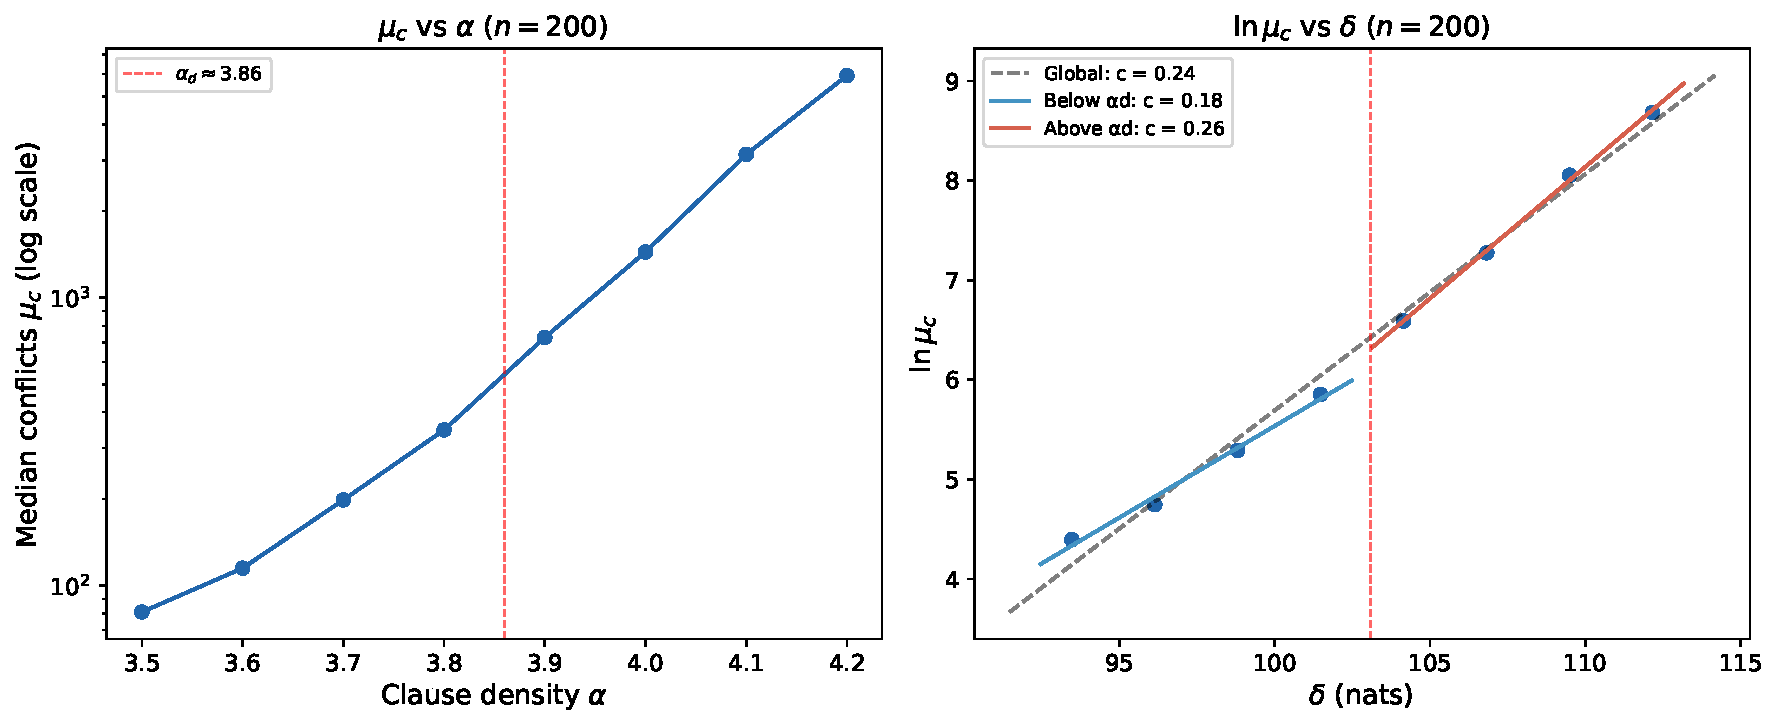
\includegraphics[width=\textwidth]{fig3_alpha_density.pdf}
\caption{節密度に対するCDCL中央値ランタイム（$n = 200$、$\alpha$あたり500インスタンス、$\alpha = 3.5$--$4.2$）。
左：対数スケールでの$\mc$。
右：区分線形フィット付き$\ln \mc$対$\delta$（$\alpha_d$以下で$c = 0.18$、以上で$c = 0.26$）。
垂直破線は$\alpha_d \approx 3.86$を示す。}
\label{fig:alpha_density}
\end{figure}


\section{計算予算メトリクス}
\label{app:metrics}

\begin{table}[h]
\centering
\begin{tabular}{lcc}
\toprule
メトリクス & $c$（CDCL） & $R^2$ \\
\midrule
コンフリクト     & 0.194 & 0.991 \\
伝播  & 0.082 & 0.757 \\
決定     & 0.040 & 0.488 \\
\bottomrule
\end{tabular}
\caption{異なる予算メトリクスに対する感応度指数（$n = 200$）。
コンフリクトが最もクリーンな乗法的分離を与え、コンフリクトがCDCLアルゴリズムの基本的な状態遷移を表すことと整合する。}
\label{tab:metrics}
\end{table}


%=============================================
% Bibliography
\begin{thebibliography}{15}

\bibitem{MPZ2009}
M.~M\'ezard, A.~Montanari,
\textit{Information, Physics, and Computation},
Oxford University Press, 2009.

\bibitem{Achlioptas2008}
D.~Achlioptas, A.~Coja-Oghlan,
``Algorithmic barriers from phase transitions,''
\textit{Proc.\ FOCS}, pp.~793--802, 2008.

\bibitem{Ding2015}
J.~Ding, A.~Sly, N.~Sun,
``Proof of the satisfiability conjecture for large $k$,''
\textit{Proc.\ STOC}, pp.~59--68, 2015.

\bibitem{Schoening1999}
T.~Sch\"oning,
``A probabilistic algorithm for $k$-SAT and constraint
satisfaction problems,''
\textit{Proc.\ FOCS}, pp.~410--414, 1999.

\bibitem{Gomes2000}
C.~P.~Gomes, B.~Selman, N.~Crato, H.~Kautz,
``Heavy-tailed phenomena in satisfiability and constraint
satisfaction problems,''
\textit{J.~Automated Reasoning}, 24(1/2):67--100, 2000.

\bibitem{Coarfa2003}
C.~Coarfa, D.~D.~Demopoulos, A.~San~Miguel~Aguirre, D.~Subramanian, M.~Y.~Vardi,
``Random 3-SAT: The plot thickens,''
\textit{Constraints}, 8(3):243--261, 2003.

\bibitem{MuHoos2015}
Z.~Mu, H.~H.~Hoos,
``On the empirical time complexity of random 3-SAT at the phase transition,''
\textit{Proc.\ IJCAI}, pp.~367--373, 2015.

\bibitem{Hoos1999}
H.~H.~Hoos, T.~St\"utzle,
``Towards a characterisation of the behaviour of stochastic local
search algorithms for SAT,''
\textit{Artificial Intelligence}, 112(1--2):213--232, 1999.

\bibitem{Frost1997}
D.~Frost, I.~Rish, L.~Vila,
``Summarizing CSP hardness with continuous probability distributions,''
\textit{Proc.\ AAAI}, pp.~327--333, 1997.

\bibitem{Aczel1966}
J.~Acz\'el,
\textit{Lectures on Functional Equations and Their Applications}.
Academic Press, 1966.

\bibitem{CoccoMonasson2001}
S.~Cocco, R.~Monasson,
``Trajectories in phase diagrams, growth processes, and
computational complexity: How search algorithms solve the
3-satisfiability problem,''
\textit{Physical Review Letters}, 86(8):1654--1657, 2001.

\bibitem{MarquesSilva1999}
J.~P.~Marques-Silva, K.~A.~Sakallah,
``GRASP: A search procedure for propositional satisfiability,''
\textit{IEEE Transactions on Computers}, 48(5):506--521, 1999.

\bibitem{SKC1994}
B.~Selman, H.~A.~Kautz, B.~Cohen,
``Noise strategies for improving local search,''
\textit{Proc.\ AAAI}, pp.~337--343, 1994.

\bibitem{BenSasson2001}
E.~Ben-Sasson, A.~Wigderson,
``Short proofs are narrow---resolution made simple,''
\textit{Journal of the ACM}, 48(2):149--169, 2001.

\bibitem{Pipatsrisawat2011}
K.~Pipatsrisawat, A.~Darwiche,
``On the power of clause-learning SAT solvers as resolution engines,''
\textit{Artificial Intelligence}, 175(2):512--525, 2011.

\end{thebibliography}

\end{document}
